%\documentclass{report}
%\documentclass{}
\documentclass[a4paper,times,numbered,print,index, table, xcdraw]{article}

\setcounter{secnumdepth}{5}
\setcounter{tocdepth}{5}

\iffalse
\usepackage{fancyhdr}
\pagestyle{fancy}
\fancyhf{}
\lhead{\nouppercase{\rightmark} (\nouppercase{\leftmark})}
\chead{}
\rhead{\thepage}
\lfoot{}
\cfoot{}
\rfoot{}
\renewcommand{\headrulewidth}{0.4pt}
\renewcommand{\footrulewidth}{0.4pt}

\renewcommand{\chaptermark}[1]{%
\markboth{#1}{}}
\fi

\usepackage{mathtools}
%\usepackage{balance}
\usepackage{epsfig}
%\usepackage[all]{xy}
\usepackage{amsmath}
\usepackage{array}
\usepackage{float}
\usepackage{subcaption}
\usepackage{color}
\usepackage{epstopdf}
\usepackage{listings}
\usepackage{graphicx}
\usepackage{amssymb}
\usepackage{parskip}
\usepackage{pifont}% http://ctan.org/pkg/pifont
\newcommand{\cmark}{\ding{51}}%
\newcommand{\xmark}{\ding{55}}%
\usepackage{enumitem}
\usepackage{multirow}
\usepackage{url}
\usepackage{cite}
\usepackage{setspace}
\usepackage{tikz}
\usepackage{graphicx}
\usepackage[margin=2.5cm]{geometry}
\usepackage{xspace}
\usepackage{multirow}
\usepackage{booktabs}

\lstset{ %
  %basicstyle=\scriptsize,           % the size of the fonts that are used for the code
  breakatwhitespace=false,          % sets if automatic breaks should only happen at whitespace
  breaklines=true,                  % sets automatic line breaking
  %commentstyle=\color{mygreen},    % comment style
  %escapeinside={\%*}{*)},          % if you want to add LaTeX within your code
  %frame=single,                    % adds a frame around the code
  keepspaces=true,                  % keeps spaces in text, useful for keeping indentation of code (possibly needs columns=flexible)
  keywordstyle=\color{blue},        % keyword style
  language=C,                       % the language of the code
  morekeywords={},                  % if you want to add more keywords to the set
  numbers=none,                     % where to put the line-numbers; possible values are (none, left, right)
  %numbersep=5pt,                   % how far the line-numbers are from the code
  %numberstyle=\tiny\color{mygray}, % the style that is used for the line-numbers
  %rulecolor=\color{black},         % if not set, the frame-color may be changed on line-breaks within not-black text (e.g. comments (green here))
  showspaces=false,                 % show spaces everywhere adding particular underscores; it overrides 'showstringspaces'
  showstringspaces=false,           % underline spaces within strings only
  showtabs=false,                   % show tabs within strings adding particular underscores
  %stepnumber=2,                    % the step between two line-numbers. If it's 1, each line will be numbered
  %stringstyle=\color{mymauve},     % string literal style
  tabsize=2,                        % sets default tabsize to 2 spaces
  %title=\lstname                   % show the filename of files included with \lstinputlisting; also try caption instead of title
}

\usepackage{hyperref}
\hypersetup{
    colorlinks,
    citecolor=red,
    filecolor=black,
    linkcolor=blue,
    urlcolor=blue
}
\usepackage{cleveref}


\newcommand{\myparagraph}[1]{\paragraph{#1}\mbox{}\\\\}
\newcommand{\mysubparagraph}[1]{\subparagraph{#1}\mbox{}\\\\}


\newcommand{\toask}[1]{\textcolor{red}{(Q): #1}}
\newcommand{\todo}[1]{\textcolor{red}{(ToDo): #1}}
\newcommand{\tocite}{\textcolor{blue}{[citation]}}
\newcommand{\rpm}{\raisebox{.2ex}{$\scriptstyle\pm$}}

\newcommand{\dc}{\textcolor{red}{DC:}\textcolor{red}}
\newcommand{\mm}{\textcolor{blue}{}\textcolor{blue}}
\newcommand{\mc}{\textcolor{green}{}\textcolor{green}}
\newcommand{\HRule}{\rule{\linewidth}{0.5mm}} % Defines a new command for the horizontal lines, change thickness here

\let\LaTeXStandardTableOfContents\tableofcontents

\renewcommand{\tableofcontents}{%
\begingroup%
\renewcommand{\bfseries}{\relax}%
\LaTeXStandardTableOfContents%
\endgroup%
}%

\newcommand\citep[1]{(\cite{#1})}

\begin{document}


\begin{titlepage}

\center % Center everything on the page

%----------------------------------------------------------------------------------------
%	TITLE SECTION
%----------------------------------------------------------------------------------------

%\HRule \\[0.4cm]
%{ \huge \bfseries Interaction between Artificial Intelligence and Computer Architecture}\\[0.4cm] % Title of your document
%\HRule \\[1.5cm]

\HRule \\[0.4cm]
{ \huge \bfseries Kernel PCA for Word Embeddings }\\[0.4cm] % Title of your document
%{ \huge \bfseries Leveraging Artificial Intelligence Algorithms \\ to Design Hardware Prediction Mechanisms}\\[0.4cm] % Title of your document
\HRule \\[1.5cm]

\textsc{\huge \textbf{Kernel-Based Machine Learning\\and Multivariate Modeling}}\\[1.5cm]

\textsc{\huge \textbf{Half-term project}}\\[1.5cm]

\textsc{\Large \textbf{Universitat Polit\`ecnica de Catalunya}}\\[1.5cm]

%----------------------------------------------------------------------------------------
%	AUTHOR & ADVISOR(S) SECTION
%----------------------------------------------------------------------------------------

\vspace{0.8cm}
\begin{minipage}{0.4\textwidth}
\begin{flushleft} \large
\Large \emph{Authors:}\\[0.1cm]
\Large Kevin Michael Frick \\
Patrick Lutz \\
Sonia Petrini

\end{flushleft}
\end{minipage}
~
\begin{minipage}{0.4\textwidth}
\begin{flushright} \large
\Large \emph{Supervisors:} \\[0.1cm]
\Large Lluís A. Belanche \\
belanche@cs.upc.edu \\[0.1cm]
\end{flushright}
\vspace{-1.47cm}
\end{minipage}\\[3cm]

%----------------------------------------------------------------------------------------
%	LOGO SECTION
%----------------------------------------------------------------------------------------


\begin{minipage}{0.45\textwidth}
\begin{flushright}
    \includegraphics[width=\textwidth]{Figures/Cover/upc.jpeg}%\\[1cm] % Include a department/university logo - this will require the graphicx package
\end{flushright}
\end{minipage}

\vspace{1.5cm}

%----------------------------------------------------------------------------------------
%	DATE SECTION
%----------------------------------------------------------------------------------------

{\large \today}\\[2cm] % Date, change the \today to a set date if you want to be precise

%----------------------------------------------------------------------------------------

\vfill % Fill the rest of the page with whitespace

\end{titlepage}

%\onehalfspacing
%\setlength{\parskip}{0.5cm plus4mm minus3mm}

%\tableofcontents
%\listoftables
%\listoffigures

%\clearpage

\thispagestyle{plain}

\section{Abstract}
\label{chap:abstract}
Kernel Principal Component Analysis has proven to be useful in improving the understanding of semantic and syntactic rules from texts.
In the literature, kernelization has been applied prior to word embedding, to initialize the embedding layer with meaningful morphological information, or after it, to reduce the dimensionality of the embeddings. 
In this work we move from these two established methodologies, testing their robustness to a smaller training vocabulary size and to the usage of a different dataset.
We evaluate their performances for different choices of embedding dimensionalities, both qualitatively and quantitatively, by comparing our performance to the state of the art.
Our results show that using morphological information for initialization is less important when using more modern and advanced implementations of the word embedding model.
On the other hand, we show that kernel PCA can be applied to trained embeddings to effectively achieve dimensionality reduction.

\section{Introduction}
\label{chap:intro}
\subsection{Word embeddings}
A word \emph{sense} or \emph{concept} is the meaning component of a word. The \textit{relations} between the words in a text, based on syntactic and semantic properties, allow one to \textit{understand} the text, that is to learn the meanings of the words it contains. Word, sentence, and text embeddings are a class of models that allow one to quantify these relations, by means of mapping elements of \textit{natural language} to \textit{vector spaces} and define a notion of ``distance'' or ``similarity'' between words. Despite working well on large text corpora, these methods have not proven to be able to learn meaningful semantic and syntactic relations from small datasets. In fact, they take each word as an independent input ignoring the information of the words' morphology, which could indeed be precious, especially when corpora are made of many different words. 
The types of relations that can be observed between words are various. Two words could be found to be syntactically and semantically close when they are \textit{synonyms} or \textit{antonyms} for instance, or when one is a \textit{category} of the other. The underlying notion of \textit{word similarity} that we employ to define these relations is based on the concept of \textbf{$n$-gram}. This refers to a word subunit, built by breaking up the word into subsequences of $n$ letters. This allows for capturing subtler relations between words, like pairs or triplets of letters that indicate an adverb or an etymological root. 


\subsection{Aim and structure}

The works by Gupta et al. \cite{gupta_improving_2019} and by Raunak \cite{raunak_simple_2017} propose two different approaches to leverage the advantages of \textit{kernalization} to add this morphological enrichment to word embeddings tasks: respectively, applying Kernel PCA \textbf{\textit{ex ante}}, to enhance Word2vec's performance and reduce training time requirements in word representation learning, and \textbf{\textit{ex post}}, to perform dimensionality reduction on the learned embeddings. 
This project builds on their proposed methodologies, expanding the scope to the following research questions:
\begin{itemize}
    \item Would the same increased performance that the authors of \cite{gupta_improving_2019} observe be obtained with a smaller training vocabulary size, compared to the one originally used?
    \item How do the results in  \cite{raunak_simple_2017} vary with respect to how aggressive the dimensionality reduction is?
    \item Are the models' performances sensitive to hyperparameter tuning on the Word2vec model? That is, can a similar improvement as that observed in \cite{gupta_improving_2019} be obtained, without any application of kernelization, by simply using an implementation of Word2vec which trains better and faster thanks to advances in optimization techniques and hyperparameter tuning?
\end{itemize}

In order to do so, we perform our analyses on the \texttt{text} dataset, available as open access from \cite{lhoest_huggingfacedatasets_2021}.
We implement the KPCA using \texttt{scikit-learn} and leverage an implementation of  Word2vec using a different framework compared to the original studies, that is \texttt{PyTorch}. 
We believe that this could also impact our results.
Among the two word representation learning methods that were leveraged in \cite{gupta_improving_2019}, we make use of \textit{skip-gram} \cite{mikolov_efficient_2013}, which is considered \cite{mikolov_distributed_2013} to be better suited for finding meaningful relations even in small texts. 

The paper is organized as follows: first, in section \ref{chap:previous} we review the existing literature on the topic. 
Then, section \ref{chap:theory} provides a complete overview of the relevant theoretical framework.
In section \ref{chap:experiments} we thoroughly report on the methods we used, and the choices we have made in the model's implementation and present our results, while the quantitative and qualitative evaluation of performance is carried out in section \ref{chap:evaluation}.


\section{Previous work}
\label{chap:previous}

In the literature there are two main strands of research concerning the usage of KPCA for word embeddings, that is using KPCA before training, as an initialization technique, and after training, to do dimensionality reduction.

\subsection{Kernel PCA for morphological warm-start}

Using kernel PCA before training \cite{gupta_improving_2019} aims at enriching the training with additional \textbf{morphological information}, conveyed through a word similarity matrix on which kernel PCA is performed. 
This work builds on the well-established idea that subword information can be a great enrichment for learning relations between words in a text. 
This is particularly relevant for those languages in which the morphological variability is very high, as in German: in such cases, predicting new words becomes a difficult task without an understanding of the underlying morphological patterns. 
In 2016, Bojanowski et al. \cite{bojanowski_enriching_2016} proposed an extension of the \textit{skip-gram} model, which is actually based on $n$-grams instead of words. 

In the same year, the authors of a probabilistic framework for word embeddings \cite{bhatia_morphological_2016} stress how using subword information at the level of single characters could lead to the identification of spurious relations, as they could pair \textit{homonyms}, words that are spelled in a similar way but have a different meaning.

\subsection{Kernel PCA for dimensionality reduction}

On the other hand, the use of kernel PCA after training \cite{raunak_simple_2017} builds on a geometrical study of word embedding using simple PCA \cite{mu_all-but--top_2017}.
Across models, word embeddings have a large mean vector and most of their energy, after subtracting the mean, is located in a low-dimensional subspace.
This means that, in principle, it would be possible to use kernel PCA to carry out effective dimensionality reduction.
However, the authors of the study obtained mixed results when using Kernel PCA as compared to standard PCA.

Finally, as an aside, we note how kernel-based methods and word embeddings are closely related.
More recent work concerns using recurrent architectures, such as long-short-term-memory \cite{yepes_word_2017} to carry out more complex pretext tasks for word embeddings.
It has recently been shown \cite{fermanian_framing_2021} that it's possible to frame recurrent architectures as kernel methods, which makes our approach even more interesting as relations could be drawn between what our kernelization is performing and a hypothetical recurrent architecture.


\section{Theoretical background}
\label{chap:theory}
\subsection{High-dimensional word embeddings}
A very simple way to define a word embedding is the canonical \emph{vector space representation}.
Simply put, given a set of $p$ documents whose vocabulary (e.g. the set of unique words (types) used, which contains no duplicates) is composed of $n$ words, we define an embedding matrix $E \in \mathbb{R}^{n\times p}$. This matrix is such that its $i$-th row is the embedding for the $i$-th word in the vocabulary, and its entry $e_{ij}$ is 0 if and only if the $i$-th word is not present in the $j$-th document. 
If the word is present in the document, the value is non-zero and is typically calculated as \emph{term frequency} in the document times the \emph{inverse document frequency}\cite{luhn_statistical_1957}, that is the log of the inverse of the term frequency (tf-idf) across documents.
This means that a word has a high frequency in one document, the magnitude of the corresponding element increases, but it's offset if the term appears many times in general in the corpus.
This kind of method to generate word embeddings encodes information that is very specific to a corpus and is therefore used commonly for information retrieval tasks such as those carried out by the backends of search engines.
However, these are ill-suited for any kind of task where evaluating word similarity is necessary. 

By defining an appropriate \textit{similarity function} $f: \mathcal{V} \times \mathcal{V} \rightarrow [0, 1]$, it is possible to compute embeddings as ``vectors of similarities'' of words in a vocabulary.
That is, given a vocabulary $V \subset \mathcal{X}$, a word $u \in \mathcal{V}$ and a similarity function $f$ as defined above, an embedding is the vector $\mathbf{e}$ such that $e_k = f(u, v_k) \: \forall \: v_k \in V$.
The embeddings of words in $V$ form a similarity matrix $S$ so that $s_{ij} = f(v_i, v_j) \: \forall \: v_i, v_j \in V$.
This is a canonical representation of word embeddings which provides morphological information. 
In highly morphological languages, such as German, morphological information is a proxy for semantic information.
For this reason, this model for embeddings can be particularly helpful for such languages.
\subsection{Dimensionality reduction on matrices}
However, both tf-idf and similarity matrix embeddings heavily suffer from the \textbf{curse of dimensionality}, that is the embeddings are calculated on a very high-dimensional space, which will make for very sparse matrices with low information density.
Many ways have been designed to tackle this issue, from random indexing \cite{karlgren_words_2001} to dimensionality reduction.
In this work, we focus on the latter techniques.

It would be possible in principle to reduce the dimensionality of the tf-idf or similarity matrix by performing simple principal component analysis (PCA).
The basic idea of principal component analysis is to find a small number of linear combinations of the observed variables which explain most of the variation in the data.
The keyword here is \emph{linear}: performing PCA would lead to excluding a large amount of information, as there are no geometrical constraints imposed by either tf-idf or the similarity measure used \cite{arora_latent_2016}.

Kernel-based principal component analysis (kernel PCA or \textbf{KPCA}) is a kernelized version of traditional principal component analysis \cite{hastie_elements_2013}.
As with any kernelized algorithm, KPCA allows one to make use of a similarity matrix to perform  PCA in a high-dimensional feature space \emph{implicitly}, using a kernel function.
The feature space is chosen indirectly via the kernel function and should be chosen in such a way that the mapped data is linearly separable into arbitrary clusters.
Since the feature map is implicit in the kernel function, the principal components are never calculated explicitly.
Rather, what is calculated is projections of the data onto those components, be it training data or test data.

\subsection{Computational considerations on KPCA}

By computing KPCA on the word similarity matrix as defined above, one can compute an initial set of ``similarity-based embeddings'', which make use of the information on morphological relations encoded by the chosen similarity measure, and have reduced dimensionality.

In order to reduce computation time, it is possible to perform KPCA on a similarity matrix $S$ generated from a set of words that is a \textit{subset} of the full vocabulary, or example composed by the most common words. We call this set $V$, of cardinality $|V|$, and we will refer to it as the \emph{training vocabulary}. 
By performing KPCA on the matrix $S$, we obtain embeddings for the words that are in the training vocabulary.
With a slight abuse of notation, we refer to the kernel PCA matrix computed on $S$ as $K = k(S)$.

In order to define a complete set of vectors for all words in the full vocabulary, we compute the embedding for any word not in the vocabulary by projecting its similarity vector onto the kernel principal components.
Since the kernel principal components reside in the feature space, it is not possible to compute them directly, but we can project arbitrary data onto them.

\subsection{Machine learning for word embeddings}

Word2vec \cite{mikolov_efficient_2013} is a family of model architectures and optimizations that can be used to learn word embeddings from large datasets. 
Embeddings learned through Word2vec have proven to be successful on a variety of downstream natural language processing tasks.
% https://neptune.ai/blog/word-embeddings-guide
% https://adoni.github.io/2017/11/08/Word2vec-pytorch/
Learnable embeddings are based on the concept of a \emph{pretext task}, that is learning a representation of the words by subsequent iterations of gradient descent on a loss function that expresses performance on some task we are not actually interested in.
That is, instead of counting how often each word $v$ occurs near another word $u$, we train a classifier on a binary prediction task: ``is $v$ likely to show up near $u$?''.
We do not actually care about this task, but we will take the learned classifier weights as the word embeddings. The embedding layer can be initialized either with random data, as is usual with weights of neural networks, or with vectors representing some kind of injected knowledge \cite{bojanowski_enriching_2016}, in which case the model is a \emph{warm-start embedding model}.

Word2vec can use the \textit{skip-gram} model as a pretext task, or the \textit{continuous bag of words} model.
To perform our analysis we employed skip-gram, since, according to the original Word2vec paper \cite{mikolov_efficient_2013}, skip-gram works well with a small amount of training data, and represents well even rare words or phrases
Skip-grams are sentence n-grams (distinct from word n-grams, sentence n-grams are composed of words and not of letters, but the way they are built is the same) that allow tokens to be skipped. 
A skip-gram model predicts the context (or neighbors) of a word, given the word itself.

The context of a word can be represented through a set of skip-gram pairs $u_t, u_c$, where $u_c$ appears in the ``neighboring context'' of $u_t$, that is in the same sentence as $u_t$ and within a certain range.
The context words for each of the words of a sentence are defined by a \textbf{window size}.
The window size determines the span of words on either side of a target word that can be considered context words.
Tuning Word2vec parameters, such as window size, learning rate, choice of optimizer etc. is outside the scope of this paper.
We use the default parameters of the implementation we leverage, which can be shown to be optimal in practice.

\subsection{KPCA for initialization and dimensionality reduction}

Word2vec allows for specifying embedding dimensionality $p$ so that computed embeddings will reside in $\mathbb{R}^p$.
To ensure that the kernel matrix can be used to initialize Word2vec, we take only the first $p$ principal components of the ``morphological word embeddings'' that result from our kernel PCA.
It has been shown \cite{gupta_improving_2019} that initializing Word2vec embeddings of size $p$ using the $p$ kernel principal components of a word leads to more accurate embeddings since such an initialization amounts to feeding the network morphological information, then letting it infer syntactical and semantic relationships between words.
This is the first approach we experiment with, that is \emph{performing dimensionality reduction on the word similarity matrix $S \in \mathbb{R}^{n\times n}$ and using the resulting matrix $K \in \mathbb{R}^{n \times p}$ as initialization for Word2vec embeddings}, then training Word2vec after this initialization and comparing it with random initialization of the embeddings.

Furthermore, it has also been shown \cite{raunak_simple_2017} that using standard and kernel PCA is an effective way to perform dimensionality reduction on word embeddings after they have been calculated.
This way of performing dimensionality reduction amounts to finding the components of the word embedding which are most significant in the embedding space itself (in the case of PCA) or in the feature space encoded by the implicit feature map (in the case of kernel PCA).
This is the second approach we experiment with, that is \emph{performing dimensionality reduction on the learned embeddings matrix $E \in \mathbb{R}^{n \times p}$, obtaining a compressed matrix $E' \in \mathbb{R}^{n' \times p}, n' < n$} and evaluating the performance of these compressed embeddings.

The objective of this paper is to evaluate the robustness of such approaches to changes in vocabulary size, datasets, pretext tasks, and implementation frameworks, and analyze whether they can be valuable tools to reduce the number of training epochs required for meaningful embeddings.



\section{Experiments}
\label{chap:experiments}

To test our hypotheses we use the \texttt{text} dataset - available as open access from \cite{lhoest_huggingfacedatasets_2021} - composed of English Wikipedia articles.
Before performing any operation we tokenize it with the default options of the tokenizer proposed by \cite{wolf-etal-2020-transformers}, removing numbers, symbols, punctuation, and special characters. 
We also lowercase every token in order not to identify spurious morphological rules, emerging from the same word being spelled in different cases. 
In \cref{table:data} we display information on our dataset, and on the smallest one considered by \cite{gupta_improving_2019}.


\begin{table}[h!]

\centering

\begin{tabular}{|l|l|l|}
\hline
\rowcolor[HTML]{C0C0C0} 
Corpus & Corpus size & Training vocabulary size \\ \hline
\cellcolor[HTML]{C0C0C0} text & $\approx$ 1 million &  1000\\ \hline
\cellcolor[HTML]{C0C0C0} 20Newsgroups & $\approx$ 1 million & 10.000\\ \hline
\end{tabular}
\caption{Corpus and training vocabulary sizes, for our considered dataset (\texttt{text}) and the smallest corpus in \cite{gupta_improving_2019}.}
\label{table:data}
\end{table}


\subsection{KPCA for warm start}
To evaluate the first approach, we follow \cite{gupta_improving_2019} for the ex-ante usage of KPCA and leverage the \textbf{$n$-gram similarity} defined in \cref{eq:ngramsim}, where $G_1, G_2$ are the sets of $n$-grams of the two words:

\begin{equation}
    s(G1, G2) = \frac{2 | G_1 \cap G_2 |}{|G_1| + |G_2|}
    \label{eq:ngramsim}
\end{equation}

As for the choice of the kernel function $k(\cdot)$, we make use of the \textbf{Gaussian kernel}, also known as RBF kernel. We perform kernel PCA on $S$ and define our kernel matrix $K = k(S)$ so that $k_{ij} = k(\mathbf{s}_i, \mathbf{s}_j) =  \exp(-\gamma\|\mathbf{s}_i - \mathbf{s}_j\|^2)$. The kernel principal components will therefore encode the notion of morphological similarity. 

\subsubsection{Hyperparameters Tuning}
In \cite{gupta_improving_2019}, the authors set the kernel parameter to $\gamma_C = \frac{1}{|V|}$. However, they do not report on doing any optimization to tune this value.
Thus, to assess if this is indeed a good choice, we perform a \textbf{grid search} on the $\gamma$ kernel parameter, evaluating it against different embedding dimensionalities.
We use as our evaluation metric the \emph{relative error on squared cosine distance}.
That is, we take all possible pairs of word embeddings and calculate the \emph{squared cosine distance} among the two rows $s_i, s_j$ of $S$ and the two rows $k_i, k_j$ of $K$.
This results in two squared distance measures $d^2_{s} = 1 - \frac{<s_i, s_j>}{\|s_i\|\|s_j\|}, d^2_{k} = 1 - \frac{<k_i, k_j>}{\|k_i\|\|k_j\|}$.
The reason why we use \textit{cosine distance} as a benchmark, is that in high-dimensional spaces the Euclidean distance between two terms may be high, while their vector representations are actually pointing in the same direction. It is known that the \textit{cosine distance} would also be distorted by a very high number of dimensions, but this effect should be minimal for the dimensionalities we are considering.
So, taking $d^2_{s}$ as the distance which encodes the most information and $d^2_k$ as an ``estimate'' of it,  we calculate the relative error as 

\begin{equation}
    \eta = \frac{|d^2_{k} - d^2_{s}|}{d^2_{s}}
\end{equation}

and then take the average out of all the values. We test parameters in the interval $[10^{-6}, 10^{-2}]$, and we compare the performance of each of these values for a range of dimensionalities, defined as $[32,64,128,256,512]$. 
This results in the parameter grid in \cref{table:cos-err-kpre}. 
N/A values correspond to cases in which a kernel PCA could not be computed due to numerical issues.
As we can see, according to this measure, performing kernel PCA on our training vocabulary similarity matrix $S$ seems to be relatively \textit{insensitive} to the choice of $\gamma$.
We therefore pick $\gamma = \frac{1}{|V|}$ as in \cite{gupta_improving_2019}.


%% OK 02.07
\begin{table}[h!]

\centering

\begin{tabular}{|l|l|l|l|l|l|}
\hline
\rowcolor[HTML]{C0C0C0} 
$(\gamma, p)$ & 32 &  64 &  128 &  256 &  512 \\ \hline
\cellcolor[HTML]{C0C0C0}$10^{-6}$& 0.195 & 0.107 & 0.056 & 0.031 & 0.017 \\ \hline
\cellcolor[HTML]{C0C0C0}$0.0005$&0.195 & 0.107 & 0.056 & 0.031 & N/A\\ \hline
\cellcolor[HTML]{C0C0C0}$0.0011$&0.195 & 0.107 & 0.056 & 0.031 & 0.017 \\ \hline
\cellcolor[HTML]{C0C0C0}$0.0016$&0.195 & 0.107 & 0.056 & 0.031 & 0.017 \\ \hline
\cellcolor[HTML]{C0C0C0}$0.0021$&0.196 & 0.107 & 0.056 & 0.031 & N/A\\ \hline
\cellcolor[HTML]{C0C0C0}$0.0026$&0.196 & 0.108 & 0.056 & 0.031 & 0.017 \\ \hline
\cellcolor[HTML]{C0C0C0}$0.0032$&0.196 & 0.108 & 0.057 & 0.031 & 0.017 \\ \hline
\cellcolor[HTML]{C0C0C0}$0.0037$&0.196 & 0.108 & 0.057 & 0.031 & 0.017 \\ \hline
\cellcolor[HTML]{C0C0C0}$0.0042$&0.196 & 0.108 & 0.057 & 0.031 & 0.017 \\ \hline
\cellcolor[HTML]{C0C0C0}$0.0047$&0.196 & 0.108 & 0.057 & 0.031 & N/A\\ \hline
\cellcolor[HTML]{C0C0C0}$0.0053$&0.196 & 0.108 & 0.057 & 0.031 & 0.018 \\ \hline
\cellcolor[HTML]{C0C0C0}$0.0057$&0.197 & 0.108 & 0.057 & 0.031 & 0.018 \\ \hline
\cellcolor[HTML]{C0C0C0}$0.0063$&0.197 & 0.109 & 0.057 & 0.032 & N/A\\ \hline
\cellcolor[HTML]{C0C0C0}$0.0068$&0.197 & 0.109 & 0.057 & 0.032 & 0.018 \\ \hline
\cellcolor[HTML]{C0C0C0}$0.0074$&0.197 & 0.109 & 0.057 & 0.032 & 0.018 \\ \hline
\cellcolor[HTML]{C0C0C0}$0.0079$&0.197 & 0.109 & 0.057 & 0.032 & 0.018 \\ \hline
\cellcolor[HTML]{C0C0C0}$0.0084$&0.197 & 0.109 & 0.057 & 0.032 & N/A\\ \hline
\cellcolor[HTML]{C0C0C0}$0.0089$&0.197 & 0.109 & 0.057 & 0.032 & 0.018 \\ \hline
\cellcolor[HTML]{C0C0C0}$0.0095$&0.197 & 0.109 & 0.058 & 0.032 & 0.018 \\ \hline
\cellcolor[HTML]{C0C0C0}$10^{-2}$&0.197 & 0.109 & 0.058 & 0.032 & 0.018 \\ \hline
\end{tabular}

\caption{\textit{Ex-ante} KPCA: \textbf{grid search} for $\gamma$ parameter of kernel function, scored according to relative error in squared \textit{cosine distance} between the same pair of words, in the original similarity matrix (S) and in the Kernel matrix (K). The lower, the better.}
\label{table:cos-err-kpre}
\end{table}

 
Although we deliberately did not perform \textbf{cross-validation}, since our purpose is fitting the studied corpus the best we can, over-fitting the information contained in the training vocabulary is still a risk. Thus, we implement this procedure with a number of folds equal to 5: however, using relative error on cosine distance as an evaluation metric is problematic in this situation, since many zero-vectors can appear in the case of words in the test fold that have no $n$-grams in common with any of the words in the training folds. This does not happen when the whole matrix is evaluated, since every vector has at least one non-zero element, corresponding to the value of the word's similarity to itself, that is 1.

We therefore review the relevant literature and find \cite{alam_hyperparameter_2014} that a metric that can be used for cross-validation on kernel PCA is the \textbf{reconstruction error}.
The reconstruction error is calculated after fitting a kernel PCA, by attempting to reconstruct the source data using only the first $p$ kernel principal components, and calculating the mean squared error between this reconstruction and the original matrix \cite{mika_fisher_1999}.

Again, we test 20 equally spaced values of $\gamma$ in the interval $[10^{-6}, 10^{-2}]$.
We calculate the root of the MSE and normalize it by dividing it by the mean value of $S$, obtaining the normalized root-mean-square-error (NRMSE).
This search confirms our hypothesis on the low sensitivity to this hyperparameter, resulting in the same array of NRMSE values regardless of the value of $\gamma$, which we report in \cref{table:nmrse-pre}.
For the sake of clarity, we round our values to the fourth decimal digit.


%% OK 01.09
\begin{table}[h!]

\centering

\begin{tabular}{|l|l|l|l|l|l|l|l|l|l|l|l|l|l|l|l|}
\hline
\rowcolor[HTML]{C0C0C0} 
Dimensionality & 32 & 64 & 128 & 256 & 512 \\ \hline
NRMSE & 6.132 & 5.349 & 4.440 & 3.419 & 2.863 \\ \hline
\end{tabular}
\caption{\textit{Ex-ante} KPCA: \textbf{cross-validated grid search}, for embedding dimensionality and $\gamma$ parameter, according to normalized root-mean-squared reconstruction error . The values are the same for the 20 values of $\gamma$ we tried. (lower is better)}
\label{table:nmrse-pre}
\end{table}
 
In \cref{fig:scree_ante} we show a scatter plot of the reconstruction NRMSE for the different dimensionality values.
We can observe how reconstruction NRMSE initially decreases steeply, to then become flatter: the breakpoint seems to be at 128 components, after which the increase in dimensionality is greater than the gain in accuracy. Hence, the authors' choice of retaining 128 components seems a reasonable compromise between error and variance.

\subsubsection{Training}

To train Word2vec, we use the sparse Adam optimizer with a cosine annealing law of learning rate decay, as proposed in \cite{loshchilov_sgdr_2016}. 
As a reminder, we are testing the robustness of the architectures proposed in \cite{gupta_improving_2019} with a different, more time-efficient implementation of Word2vec\footnote{\url{https://github.com/Andras7/Word2vec-pytorch}} and a smaller vocabulary. To do so, we perform KPCA on a similarity matrix generated using the 1000 most common words in the dataset. Notice that, after we select these 1000 words, we apply a filter to remove occurrences with less than 3 letters, due to our similarity measure being based on \textit{3-grams}.

We train Word2vec initializing the embeddings with either our computed KPCA-based embeddings representing morphological similarity or random data uniformly distributed in $[-\frac{1}{p}, \frac{1}{p}]$. Both times, the model is trained for 3 epochs on the entire training set using the skip-gram model as a pretext task.
To conceive a qualitative idea of the obtained embeddings, in \cref{table:5nn-1k-pre}, we show the \textbf{5 Nearest Neighbors} of 5 different words - chosen for illustrative purposes - as identified by the KPCA-initialized and the random-initialized Word2vec, for different training times. 

%% OK 02.19

\begin{table}[h!]
\begin{tabular}{|l|l|l|}
\hline
\rowcolor[HTML]{C0C0C0} 
\textbf{Word}  & \textbf{Model}          & \textbf{5-NN} \\ \hline
history &       KPCA, no further training & 'story', 'historia', 'tory', 'prehistory', 'storz'\\ \hline 
history        & KPCA, 1 epoch & 'era', 'compiled', 'sporting', 'eighteenth', 'achievements'\\ \hline
history        & KPCA, 3 epochs & 'milestone', 'selborne', 'histories', 'arguably', 'milestones'\\ \hline
history        & Word2vec, 1 epoch      &'era', 'compiled', 'sporting', 'achievements', 'chess' \\ \hline
history        & Word2vec, 3 epochs       &'selborne', 'histories', 'milestones', 'milestone', 'triumphs' \\ \hline
moscow         & KPCA, no further training & 'moscoso', 'discos', 'mosley', 'deimos', 'mimosa' \\ \hline
moscow         & KPCA, 1 epoch & 'vienna', 'luxembourg', 'warsaw', 'czechoslovakia', 'buenos'\\ \hline
moscow         & KPCA, 3 epochs & 'munich', 'zürich', 'prague', 'bucharest', 'warsaw' \\ \hline
moscow         & Word2vec, 1 epoch      & 'vienna', 'luxembourg', 'warsaw', 'munich', 'czechoslovakia'\\ \hline
moscow         & Word2vec, 3 epochs       & 'prague', 'zürich', 'munich', 'bucharest', 'zurich' \\ \hline
linguistically & KPCA, no further training & 'recalling', 'hallingskeid', 'victualling', 'pallingham', 'footballing'\\ \hline
linguistically & KPCA, 1 epoch & 'equine', 'homotopy', 'coexisted', 'evolutionarily', 'qualitative'\\ \hline
linguistically & KPCA, 3 epochs & 'polytheistic', 'abrahamic', 'shaivism', 'daoism', 'cognates'\\ \hline
linguistically & Word2vec, 1 epoch      &'equine', 'salvia', 'coexisted', 'homotopy', 'psychoactive' \\ \hline
linguistically & Word2vec, 3 epochs     & 'polytheistic', 'shaivism', 'daoism', 'usages', 'heathens'\\ \hline
statistics     & KPCA, no further training & 'statistic', 'ecstatic', 'statistician', 'batista', 'statisticians'\\ \hline
statistics     & KPCA, 1 epoch & 'statistical', 'nationally', 'competitive', 'selection', 'scholarships'\\ \hline
statistics     & KPCA, 3 epochs & 'statistical', 'statistic', 'stats', 'cumulative', 'statistically'\\ \hline
statistics     & Word2vec, 1 epoch     & 'statistical', 'competitive', 'nationally', 'eligibility', 'unprecedented'\\ \hline
statistics     & Word2vec, 3 epochs       & 'statistical', 'statistic', 'stats', 'cumulative', 'milestones'\\ \hline
firecracker    & KPCA, no further training & 'firecrackers', 'backfire', 'adirondacks', 'adirondack', 'dirac'\\ \hline
firecracker    & KPCA, 1 epoch & 'pushy', 'neologisms', 'rumba', 'moppet', 'munsey' \\ \hline
firecracker    & KPCA, 3 epochs & 'mashing', 'shrieking', 'jackhammer', 'jittery', 'disarmingly' \\ \hline
firecracker    & Word2vec, 1 epoch      &'marcas', 'congreve', 'opiate', 'inheritances', 'humourless' \\ \hline
firecracker    & Word2vec, 3 epochs       & 'jittery', 'mashing', 'jackhammer', 'outshines', 'shrieking' \\ \hline
\end{tabular}
\caption{\textit{Ex-ante} KPCA: Comparison of KPCA-initalized and random-initialized Word2vec in identifying \textbf{5 Nearest Neighbors} of a set of words, using embeddings in $\mathbb{R}^{128}$. Results are shown for different training epochs, namely 0 (for KPCA), 1, and 3.}
\label{table:5nn-1k-pre}
\end{table}

Furthermore, we evaluate the performance of our embeddings in a \textbf{word matching} task,  similar to that carried out in \cite{mikolov_efficient_2013}, that is minimizing the distance between words that are related in meaning but serve different syntactical purposes. For the purposes of this work, we pick cosine distance in \textit{adjective-adverb} pairs. We report our findings in \cref{table:synmatch-1k-pre} and \cref{fig:cos_dist_ante}.

Finally, we also perform a quantitative evaluation of injecting morphological knowledge obtained by fitting a kernel PCA. We use the framework in \cite{conneau_senteval_2018}, which tests the performance of the computed word embeddings using different semantic textual similarity (STS) tasks, then calculates the \textbf{Spearman correlation coefficient} between the metrics obtained by our embeddings and those computed by state-of-the-art models. A higher correlation coefficient means our embeddings are closer to the state of the art. 

We report our results in \cref{table:quant-1k-pre}.

%% OK 02.19

\begin{table}[H]

\centering

\begin{tabular}{|l|l|l|}
\hline
\rowcolor[HTML]{C0C0C0} 
\textbf{Pair}  & \textbf{Model}          & \textbf{Squared Cosine Distance}                                                             \\ \hline
quick, quickly & KPCA, no further training & 0.0004\\ \hline
quick, quickly & KPCA, 1 epoch & 0.496\\ \hline
quick, quickly & KPCA, 3 epochs & 0.690\\ \hline
quick, quickly & Word2vec, 1 epoch & 0.494\\ \hline
quick, quickly & Word2vec, 3 epochs & 0.679\\ \hline
statistical, statistically & KPCA, no further training & 0.199\\ \hline
statistical, statistically & KPCA, 1 epoch & 0.222\\ \hline
statistical, statistically & KPCA, 3 epochs & 0.334\\ \hline
statistical, statistically & Word2vec, 1 epoch & 0.228\\ \hline
statistical, statistically & Word2vec, 3 epochs & 0.356\\ \hline
calm, calmly & KPCA, no further training & 0.003 \\ \hline
calm, calmly & KPCA, 1 epoch & 0.176\\ \hline
calm, calmly & KPCA, 3 epochs &0.434 \\ \hline
calm, calmly & Word2vec, 1 epoch & 0.195\\ \hline
calm, calmly & Word2vec, 3 epochs & 0.425\\ \hline
thorough, thoroughly & KPCA, no further training & 0.0002\\ \hline
thorough, thoroughly & KPCA, 1 epoch & 0.138\\ \hline
thorough, thoroughly & KPCA, 3 epochs & 0.530\\ \hline
thorough, thoroughly & Word2vec, 1 epoch & 0.150\\ \hline
thorough, thoroughly & Word2vec, 3 epochs & 0.543\\ \hline
\end{tabular}
\caption{\textit{Ex-ante} KPCA: Comparison of KPCA-initalized and random-initialized Word2vec in \textbf{word matching tasks}: adjective-adverb matching, scored according to squared cosine distance (lower is better).}
\label{table:synmatch-1k-pre}
\end{table}


%% OK 02.19

\begin{table}[h]

\centering

\begin{tabular}{|l|l|l|}
\hline
\rowcolor[HTML]{C0C0C0} 
\textbf{Model}          & \textbf{Spearman correlation coefficient} \\ \hline
KPCA warm-start, no further training & 0.307 \\ \hline
KPCA warm-start, 1 epoch & 0.445 \\ \hline
Word2vec, 1 epoch & 0.447 \\ \hline
KPCA warm-start, 2 epochs  & 0.481 \\ \hline
Word2vec, 2 epochs &  0.490 \\ \hline
KPCA warm-start, 3 epochs &  0.508 \\ \hline
Word2vec, 3 epochs & 0.518\\ \hline
\end{tabular}
\caption{\textit{Ex-ante} KPCA: Comparison of KPCA-initalized and random-initialized Word2vec in \textbf{Spearman correlation coefficient} (higher is better).}
\label{table:quant-1k-pre}
\end{table}

From the table, a flaw emerges in the tokenizer we used: ``zurich'' and ``zürich'' are considered as being different words.
Even though we specified to the tokenizer that it should strip accents, it deliberately did not consider umlauts as accents, nor does the tokenizer provide an option to explicitly strip umlauts.
However, the choice of the tokenizer's programmers makes sense in the context of a tokenizer that is to be used on many different languages.
In languages such as German, minimal pairs exist that differ in meaning while their spelling only differs because of an umlaut.
It is the case, for example, of ``Apfel'' (apple, singular) and ``Äpfel'' (apples, plural).

\subsection{KPCA for dimensionality reduction}

We choose the RBF kernel as our function to perform kernel PCA dimensionality reduction on Word2vec embeddings, trained with a cold start.
In order to reduce computation time, we perform kernel PCA on a training vocabulary $V$ and then project the results, as we did in the previous experiment; therefore, we use the same interval on $\gamma$ as before for our grid search.
We start from embeddings in $\mathbb{R}^{128}$ and grid search for the kernel parameter, leveraging the same two evaluation metrics as before (cosine similarity on the whole dataset, and NRMSE for cross-validation), but a more aggressive dimensionality reduction. The results are shown in the parameter grids in \cref{table:cos-err-kpost} and \cref{table:nmrse-post}. 
Once again, the kernel PCA seems to be insensitive to the parameter $\gamma$, and we therefore pick $\gamma = 1/|V|$.
In \cref{table:cos-err-kpost}, we report values for the grid search performed on embeddings obtained after three epochs. 
Values for embeddings obtained after fewer epochs confirm our findings about a low sensitivity to hyperparameters and are not reported for the sake of clarity.

We deem NRMSE search more informative since values are exactly the same across values of $\gamma$, similarly to what happens with relative error on squared cosine distance, but change significantly with the aggressiveness of dimensionality reduction and across epochs.
Therefore, we are able to plot NRMSE against dimensionality in \cref{fig:scree_post} in order to draw conclusions about the effectiveness of dimensionality reduction. The NRMSE search on dimensionality, combined with \cref{fig:scree_post}, highlights how 16 would be a reasonable choice for the number of dimensions to retain when only one epoch of training is allowed.

%% OK 01.09
\begin{table}[H]

\centering

\begin{tabular}{|l|l|l|l|l|}
\hline
\rowcolor[HTML]{C0C0C0} 
Dimensionality & 8 & 16 & 32 & 64  \\ \hline
\cellcolor[HTML]{C0C0C0}Relative error in squared cosine distance & 0.276 & 0.182 & 0.120 & 0.083 \\ \hline
\end{tabular}

\caption{\textit{ex-post} KPCA: \textbf{grid search} for $\gamma$ parameter of kernel function, scored according to relative error in squared \textit{cosine distance} between the same pair of words, in the original embedding matrix (E) and in the Kernel matrix (K). These values are the same for the 20 equally-spaced values of $\gamma \in [10^{-6}, 10^{-2}]$}
\label{table:cos-err-kpost}
\end{table}







%% OK 01.09
\begin{table}[h!]

\centering

\begin{tabular}{|l|l|l|l|l|l|l|l|l|l|l|l|l|l|l|l|}
\hline
\rowcolor[HTML]{C0C0C0} 
Dimensionality & 8 & 16 & 32 & 64  \\ \hline
\cellcolor[HTML]{C0C0C0}NRMSE, 1 epoch & 13.5 & 11.5 & 9.59 & 8.27  \\ \hline
\cellcolor[HTML]{C0C0C0}NRMSE, 2 epochs & 15.4 & 14.0 & 12.0 & 9.0  \\ \hline
\cellcolor[HTML]{C0C0C0}NRMSE, 3 epochs & 17.8 & 16.5 & 14.8 & 11.7  \\ \hline

\end{tabular}
\caption{Normalized root-mean-squared error obtained with each embedding dimensionality, for models trained for a different amount of epochs. The values are the same for the 20 values of $\gamma$ we tried.}
\label{table:nmrse-post}
\end{table}

We perform KPCA to do dimensionality reduction of the embeddings to $\mathbb{R}^k, k \in \{8, 16, 32, 64\}$ and report an evaluation table based on the 5 nearest neighbors in \cref{table:5nn-1k-post}. We also report our finding on adjective-adverb matching in \cref{table:synmatch-post}. Finally, in \cref{table:quant-1k-post} we display a quantitative comparison table that uses the same tasks as our ex-ante KPCA, analyzing how different degrees of dimensionality reduction affect the performance of our model.

%% OK 01.40

\begin{table}[h]
\begin{tabular}{|l|l|l|}
\hline
\rowcolor[HTML]{C0C0C0} 
\textbf{Word}  & \textbf{Model}          & \textbf{5-NN}                                                             \\ \hline
% history & KPCA in $\mathbb{R}^{8}$ & 'era', 'biennial', 'usila', 'polled', 'bantam'\\ \hline
history & KPCA in $\mathbb{R}^{16}$ & 'era', 'bantam', 'eclipsed', 'seventeenth', 'calendar' \\ \hline
% history & KPCA in $\mathbb{R}^{32}$ & 'olympiad', 'preeminent', 'milestone', 'arguably', 'accomplishments'\\ \hline
% history & KPCA in $\mathbb{R}^{64}$ &  'milestones', 'milestone', 'selborne', 'histories', 'significance'\\ \hline
history & Original in $\mathbb{R}^{128}$ & 'selborne', 'histories', 'milestones', 'milestone', 'triumphs'\\ \hline
% moscow & KPCA in $\mathbb{R}^{8}$ & 'luxembourg', 'triumvirate', 'alliance', 'takeover', 'zürich'\\ \hline
moscow & KPCA in $\mathbb{R}^{16}$ & 'zürich', 'petrograd', 'yalta', 'zurich', 'munich' \\ \hline
% moscow & KPCA in $\mathbb{R}^{32}$ & 'munich', 'prague', 'zürich', 'zurich', 'bucharest'\\ \hline
% moscow & KPCA in $\mathbb{R}^{64}$ & 'prague', 'munich', 'zürich', 'bucharest', 'warsaw' \\ \hline
moscow & Original in $\mathbb{R}^{128}$ & 'prague', 'zürich', 'munich', 'bucharest', 'zurich'\\ \hline
% linguistically & KPCA in $\mathbb{R}^{8}$ & 'kosher', 'grammars', 'usages', 'propagating', 'cultivating' \\ \hline
linguistically & KPCA in $\mathbb{R}^{16}$ & 'shaivism', 'daoism', 'orcadian', 'polytheistic', 'interchangeably'\\ \hline
% linguistically & KPCA in $\mathbb{R}^{32}$ & 'daoism', 'polytheistic', 'shaivism', 'abrahamic', 'heathens' \\ \hline
% linguistically & KPCA in $\mathbb{R}^{64}$ & 'polytheistic', 'shaivism', 'daoism', 'heathens', 'abrahamic'\\ \hline
linguistically & Original in $\mathbb{R}^{128}$ & 'polytheistic', 'shaivism', 'daoism', 'usages', 'heathens' \\ \hline
% statistics & KPCA in $\mathbb{R}^{8}$ & 'ipc', 'partnerships', 'federations', 'nordic', 'sponsors'\\ \hline
statistics & KPCA in $\mathbb{R}^{16}$ & 'statistical', 'voting', 'selection', 'competitiveness', 'regulation'\\ \hline
% statistics & KPCA in $\mathbb{R}^{32}$ & 'statistical', 'statistic', 'benchmark', 'proficiency', 'statistically' \\ \hline
% statistics & KPCA in $\mathbb{R}^{64}$ & 'statistical', 'statistic', 'stats', 'cumulative', 'milestones'\\ \hline
statistics & Original in $\mathbb{R}^{128}$ & 'statistical', 'statistic', 'stats', 'cumulative', 'milestones'\\ \hline
% firecracker & KPCA in $\mathbb{R}^{8}$ &'callback', 'charizard', 'scintillating', 'junkies', 'lithe'\\ \hline
firecracker & KPCA in $\mathbb{R}^{16}$ & 'junkies', 'glitz', 'mashing', 'kiddie', 'stringing' \\ \hline
% firecracker & KPCA in $\mathbb{R}^{32}$ & 'mashing', 'glitz', 'outshines', 'jittery', 'daydreaming'\\ \hline
% firecracker & KPCA in $\mathbb{R}^{64}$ & 'mashing', 'jittery', 'outshines', 'jackhammer', 'shrieking'\\ \hline
firecracker & Original in $\mathbb{R}^{128}$ & 'jittery', 'mashing', 'jackhammer', 'outshines', 'shrieking'\\ \hline
\end{tabular}
\caption{\textit{Ex-post} KPCA: comparison of KPCA-compressed embeddings in $\mathbb{R}^{16}$, and original embeddings in identifying \textbf{5 Nearest Neighbors} of a set of words.}
\label{table:5nn-1k-post}
\end{table}

%% OK 01.37

\begin{table}[h]

\centering

\begin{tabular}{|l|l|l|}
\hline
\rowcolor[HTML]{C0C0C0} 
\textbf{Pair}  & \textbf{Model} & \textbf{Squared Cosine Distance} \\ \hline
quick, quickly & KPCA in $\mathbb{R}^{8}$       & 0.559  \\ \hline
quick, quickly & KPCA in $\mathbb{R}^{16}$      & 0.656  \\ \hline
quick, quickly &  KPCA in $\mathbb{R}^{32}$     & 0.698  \\ \hline
quick, quickly &  KPCA in $\mathbb{R}^{64}$     &  0.685 \\ \hline
quick, quickly & Original in $\mathbb{R}^{128}$ &  0.680 \\ \hline
statistical, statistically & KPCA in $\mathbb{R}^{8}$       & 0.467   \\ \hline
statistical, statistically & KPCA in $\mathbb{R}^{16}$      & 0.298  \\ \hline
statistical, statistically &  KPCA in $\mathbb{R}^{32}$     & 0.371  \\ \hline
statistical, statistically &  KPCA in $\mathbb{R}^{64}$     & 0.382   \\ \hline
statistical, statistically & Original in $\mathbb{R}^{128}$ & 0.355  \\ \hline
calm, calmly & KPCA in $\mathbb{R}^{8}$       & 0.206  \\ \hline
calm, calmly & KPCA in $\mathbb{R}^{16}$      & 0.315   \\ \hline
calm, calmly &  KPCA in $\mathbb{R}^{32}$     & 0.387  \\ \hline
calm, calmly &  KPCA in $\mathbb{R}^{64}$     & 0.428  \\ \hline
calm, calmly & Original in $\mathbb{R}^{128}$ & 0.424  \\ \hline
thorough, thoroughly & KPCA in $\mathbb{R}^{8}$       & 0.521   \\ \hline
thorough, thoroughly & KPCA in $\mathbb{R}^{16}$      & 0.554   \\ \hline
thorough, thoroughly &  KPCA in $\mathbb{R}^{32}$     & 0.565  \\ \hline
thorough, thoroughly &  KPCA in $\mathbb{R}^{64}$     & 0.566   \\ \hline
thorough, thoroughly & Original in $\mathbb{R}^{128}$ & 0.543  \\ \hline

\end{tabular}
\caption{\textit{ex-post} KPCA: comparison of KPCA-compressed embeddings and original embeddings in \textbf{word matching tasks},  scored according to squared cosine distance: KPCA is evaluated for various degrees of dimensionalities, namely $\{8,16,32,64\}$.}
\label{table:synmatch-post}
\end{table}


%% OK 01.37

\begin{table}[h]

\centering

\begin{tabular}{|l|l|l|}
\hline
\rowcolor[HTML]{C0C0C0} 
\textbf{Dimensionality} & \textbf{Spearman correlation coefficient} \\ \hline
KPCA in $\mathbb{R}^8$ , 1 epoch & 0.418 \\ \hline
KPCA in $\mathbb{R}^{16}$, 1 epoch & 0.436 \\ \hline
KPCA in $\mathbb{R}^{32}$, 1 epoch & 0.427 \\ \hline
KPCA in $\mathbb{R}^{64}$, 1 epoch & 0.412 \\ \hline
Original in $\mathbb{R}^{128}$, 1 epoch & 0.447 \\ \hline
KPCA in $\mathbb{R}^8$ , 2 epochs & 0.431 \\ \hline
KPCA in $\mathbb{R}^{16}$, 2 epochs & 0.476 \\ \hline
KPCA in $\mathbb{R}^{32}$, 2 epochs & 0.481 \\ \hline
KPCA in $\mathbb{R}^{64}$, 2 epochs & 0.479 \\ \hline
Original in $\mathbb{R}^{128}$, 2 epochs & 0.490 \\ \hline
KPCA in $\mathbb{R}^8$ , 3 epoch & 0.433\\ \hline
KPCA in $\mathbb{R}^{16}$, 3 epochs & 0.477 \\ \hline
KPCA in $\mathbb{R}^{32}$, 3 epochs & 0.490\\ \hline
KPCA in $\mathbb{R}^{64}$, 3 epochs & 0.506\\ \hline
Original in $\mathbb{R}^{128}$, 3 epochs & 0.518 \\ \hline
\end{tabular}
\caption{\textit{Ex-post} KPCA: \textbf{Spearman correlation coefficient} of original embeddings and KPCA embeddings, for various degrees of dimensionality reduction (higher is better). }
\label{table:quant-1k-post}
\end{table}



\section{Evaluation}
\label{chap:evaluation}
\subsection{KPCA for warm start}

\subsubsection{Qualitative performance}
Our qualitative evaluation in \cref{table:5nn-1k-pre} shows that, for common words, KPCA initialization is able to place very uncommon words next to their morphological cognates, while cold-start Word2vec is completely off the track initially but catches up after some training. For example, a cold-start model places common words such as ``history'' near related words such as ``legacy'' after one iteration but fails to learn coherent neighbors for more uncommon words, such as ``firecracker'' unless further training is carried out.

The initial performance is not on par with what is reported in \cite{gupta_improving_2019}, which suggests vocabulary size plays a significant role in the quality of morphological word embeddings. We find that after just one epoch, semantic information encoded by Word2vec entirely takes precedence, and the model disregards the morphological information encoded in the initial start. Moreover, the quality of the cold-start embeddings after one epoch is better than what the authors have found in \cite{gupta_improving_2019}, which is probably to be attributed to a better implementation of Word2vec used in our work.

We find that, predictably, the embeddings which perform the best in syntactic matching tasks are those calculated using only kernel PCA. We can see this from \cref{fig:cos_dist_ante}: at 0 epochs (meaning KPCA without further training), the squared cosine distance is almost 0, with the curious exception of "statistical-statistically". 
This is due to the high morphological similarity of adjectives and their related adverbs in English.
However, we also see that, for a vocabulary size of the order of 1000, in such morphology-related tasks initializing Word2vec with morphological information encoded using kernel PCA does not show a consistent improvement with respect to a cold-start. 

\subsubsection{Quantitative performance}
From \cref{fig:spear_ante} we can see how after one epoch, the warm-started model performs on par with a cold-start model, while the cold-start model performs better when more training is allowed. 

Therefore, we conclude that using KPCA for Word2vec warm-start may lead to better embeddings only when the training vocabulary size is large, and only a few epochs of training are allowed. Moreover, the hyperparameters in the implementation of Word2vec together with the choice of the optimizer and the learning rate decay, evidently matter more than the initialization, since the more optimized implementation we are using is able to  identify useful embeddings more quickly than what was implied by \cite{gupta_improving_2019}.

Since low-powered environments - like a laptop computer- usually restrict memory usage as well as training time, the trade-off is worth it if fitting a kernel PCA on a large vocabulary translates into saving a significant amount of time compared to further training of Word2vec.
Furthermore, \textbf{depending on the task at hand}, warm-start Word2vec embeddings might prove more suitable, as shown by our syntactic matching example, where embeddings initialized with a kernel PCA lose less accuracy in adjective-adverb matching when they are trained.




\subsection{KPCA for dimensionality reduction}


We see that performing very aggressive dimensionality reduction, such as moving from 128 to 8 dimensions, leads to embeddings that have largely lost meaning, and are not even able to relate ``statistics'' and ``statistical''. However, we find this effect largely decreases with as few as 16 embeddings for easier and more common words, like relating Moscow to other cities. On the other hand, less common words such as ``firecracker'' need a very high dimension in order to be related to words which, if not close in meaning, make sense as context words. 

We can visualize the effects of retaining different dimensionalities in \cref{fig:scree_post} and \cref{fig:spear_post}. For the first epoch, the accuracy of the resulting embeddings strongly depends on the number of components, with 16 being the most suitable choice both according to NRMSE and Spearman correlation with state-of-the-art embeddings. However, the more we increase training time, the more the error seems to become linear in dimensionality. Thus, when there are fewer than 3 epochs of training, performing a moderately aggressive dimensionality reduction leads to better performance in syntactic matching tasks \emph{with respect to a less aggressive one}. 

This reasoning is also supported by the performance in adjective-adverb matching tasks, which we show in \cref{fig:cos_dist_post}: a moderate dimensionality reduction seems to outperform the original embeddings in $\mathbb{R}^{128}$. This suggests that performing kernel PCA might allow already-trained word embeddings to better cluster together words that are close in meaning, thanks to what the feature map is learning, at the cost of the general quality of the embedding.

\section{Conclusions}
\label{chap:conclusions}
The main goal of this work was to explore two ways of using kernel PCA for word embeddings: the idea of enriching word embeddings, generated by a skip-gram model, with morphological information, and of using kernel PCA to perform dimensionality reduction after fitting the embeddings without any initialization. In particular, we tested the robustness of these methods to a smaller training vocabulary size, exploring the effects of employing different dimensionalities and of hyperparameters tuning. 

% Would the same increased performance that the authors of \cite{gupta_improving_2019} observe be obtained with a smaller training vocabulary size, compared to the one originally used?
As expected, we found that the model in \cite{gupta_improving_2019} achieves decent accuracy in initial iterations, but that using a low vocabulary size strongly impacts the said accuracy. After a couple of epochs of training, our implementation sees the semantical information encoded by word2vec take precedence over the injected morphological information.
Therefore, \emph{the same increased performance cannot be obtained with a smaller training vocabulary size, compared to the one used in \cite{gupta_improving_2019}}.


% Are the models' performances sensitive to hyperparameter tuning on the Word2vec model? That is, can a similar improvement as that observed in \cite{gupta_improving_2019} be obtained, without any application of kernelization, by simply using an implementation of Word2vec which trains better and faster thanks to advances in optimization techniques and hyperparameter tuning?
We note that morphological information results in sensible embeddings which allow words with similar meanings to start close. We see this happening with ``statistical'' and ``stats'', for example. Therefore, we conclude that kernel PCA can be a valuable tool for warm-starting embedding models \emph{when a large vocabulary size is used}.
Computing kernel PCA is faster than training word2vec for an epoch, even if the vocabulary size is large, therefore the trade-off is acceptable.
However, we observe that \emph{a similar improvement as that observed in \cite{gupta_improving_2019} can be obtained, without any application of kernelization, by simply using a better implementation of Word2vec}.


% How do the results in  \cite{raunak_simple_2017} vary with respect to how aggressive the dimensionality reduction is?
Concerning ex-post dimensionality reduction, we find that kernel PCA is effective in reducing dimensionality, but this entails a cost in embedding accuracy.
For applications where memory or bandwidth play a crucial role, like in embedded systems, the reduction of the output embeddings could prove very useful.
By reducing the size to $1/8$ of the original 128-dimensional embedding with a size of 150MB to 16 dimensions the file size could be reduced to around 19MB with a decrease of $8\%$ or less in embedding quality (see \cref{table:quant-1k-post}).
This confirms the authors' conclusions in \cite{raunak_simple_2017} and could be used as a basis for an automatic reduction of embedding dimensionality when faced with memory constraints.
The results in \cite{raunak_simple_2017}, therefore, \emph{vary linearly with respect to dimensionality only when at least three epochs of training are allowed.}
\emph{With less training, moderately aggressive dimensionality reduction fares better than either very light or very heavy reduction.}


\textit{Future work} could expand on this topic from different perspectives. One could concern the usage of different kernels with lower-dimensional feature maps, which should however be chosen carefully, taking into account the kind of data analyzed and the scope of the analysis. Then, different criteria to build the training vocabulary could be explored: we would be interested in the effects of basing the choice not only on frequency but also on word length. This is also related to the choice of a string similarity measure. While the \textit{3-gram} similarity seems to be a very good option for English Wikipedia pages, other alternatives could be explored when dealing with other languages and corpora. Finally, an interesting expansion would imply applying both the techniques we reported here, performing KPCA both prior and posterior to word embedding.


\pagebreak
\appendix
%% REDO THE PLOTS

\section{Figures}

\subsection{\textit{Ex-ante} KPCA}
% EX ANTE
% scree ante
\begin{figure}[H]  
\centering
\includegraphics[width=12cm,height=8cm]{./Figures/scree_ante.eps}
\caption{\textit{ex-ante} KPCA: Normalized root-mean-squared reconstruction error for 1 epoch, and 32, 64, 128, 256, 512 dimensions. Lower is better.} 
\label{fig:scree_ante}
\end{figure}


% cos_dist_ante
\begin{figure}[H]  
\centering
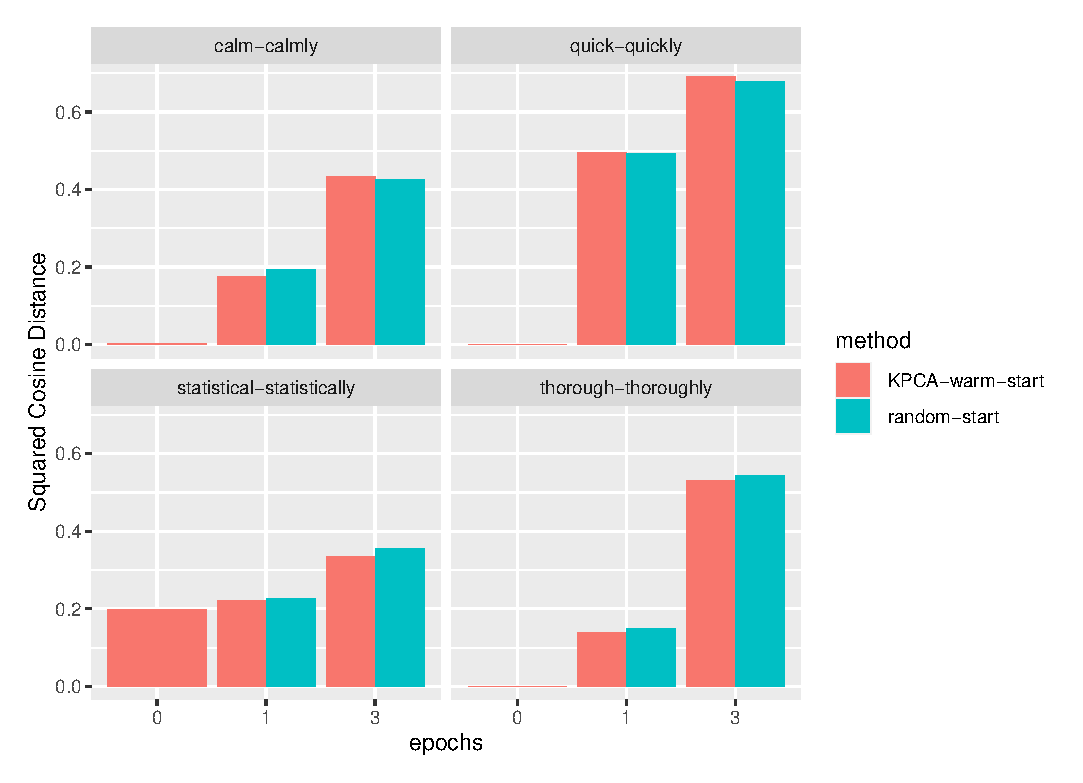
\includegraphics[width=12cm,height=9cm]{Figures/cos_dist_ante.eps}
\caption{\textit{ex-ante} KPCA: Squared cosine distance between \textbf{adjective-adverb pairs}, with KPCA-initialized (no further training, 1, 3 epochs) and random-initialized (1 and 3 epochs) word2vec. Lower is better.}
\label{fig:cos_dist_ante}
\end{figure}

% spearman
\begin{figure}[H]  
\centering
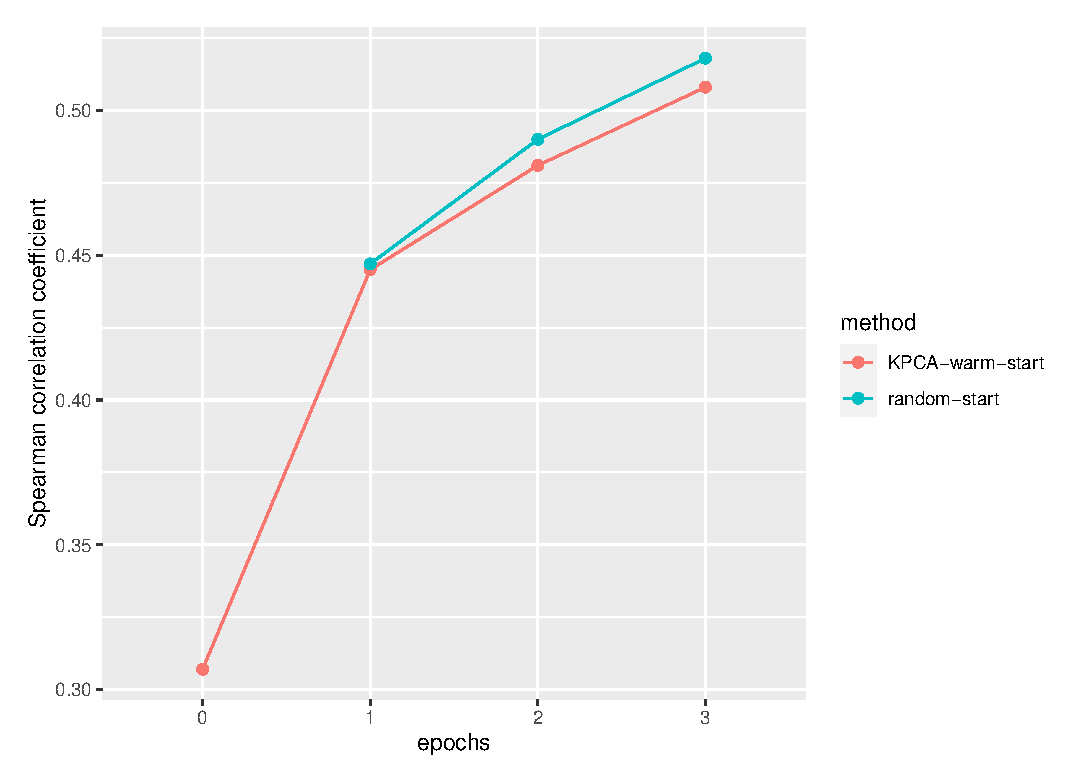
\includegraphics[width=14cm,height=10cm]{./Figures/spear_ante.eps}
\caption{\textit{ex-ante} KPCA: \textbf{Spearman correlation coefficient} of KPCA-initialized (no further training, 1, 3 epochs) and random-initialized (1 and 3 epochs) word2vec with state-of-the-art embeddings.} 
\label{fig:spear_ante}
\end{figure}





\subsection{\textit{Ex-post} KPCA}
% EX POST

% scree post
\begin{figure}[H]  
\centering
\includegraphics[width=12cm,height=8cm]{./Figures/scree_post.eps}
\caption{ \textit{ex-post} KPCA: Normalized root-mean-squared reconstruction error for 1, 2, 3 epochs, and 8, 16, 32, 64 dimensions. Lower is better.} 
\label{fig:scree_post}
\end{figure}

% cos_dist_post
\begin{figure}[H]  
\centering
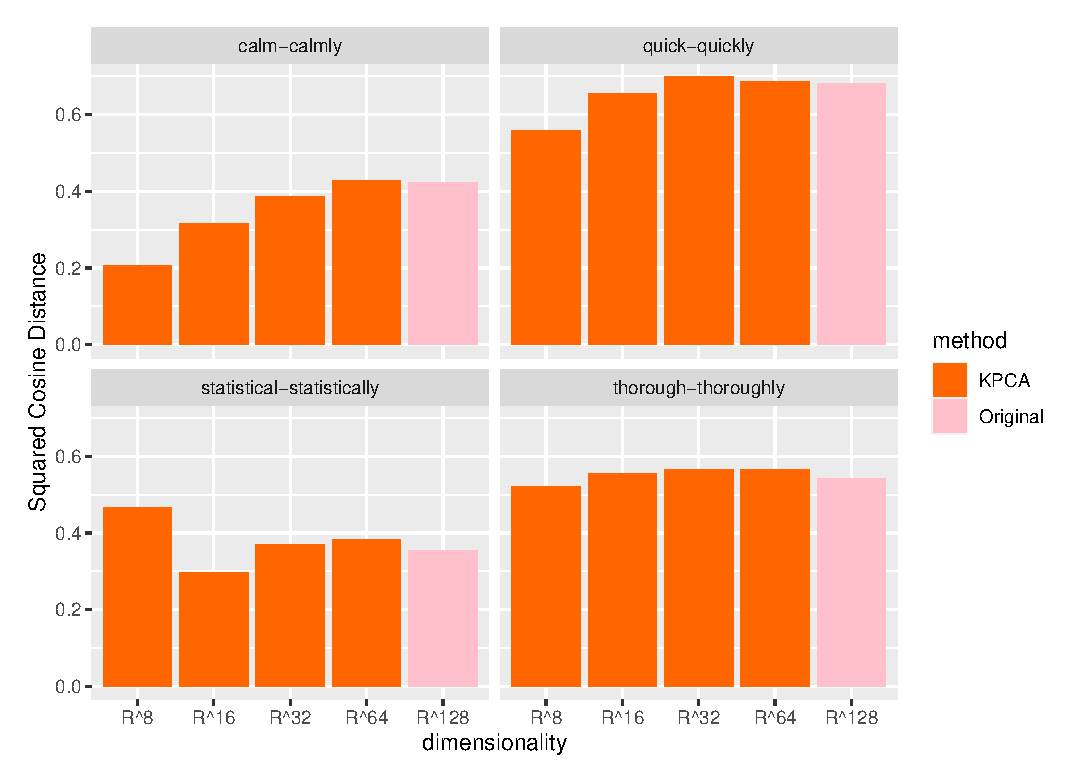
\includegraphics[width=12cm,height=9cm]{./Figures/cos_dist_post.eps}
\caption{ \textit{ex-post} KPCA: Squared cosine distance between adjective-adverb pairs, with KPCA embeddings (for 8, 16, 32, 64 dimensions) and original embeddings (in the original 128 dimensions). Lower is better.} 
\label{fig:cos_dist_post}
\end{figure}


% spearman
\begin{figure}[H]  
\centering
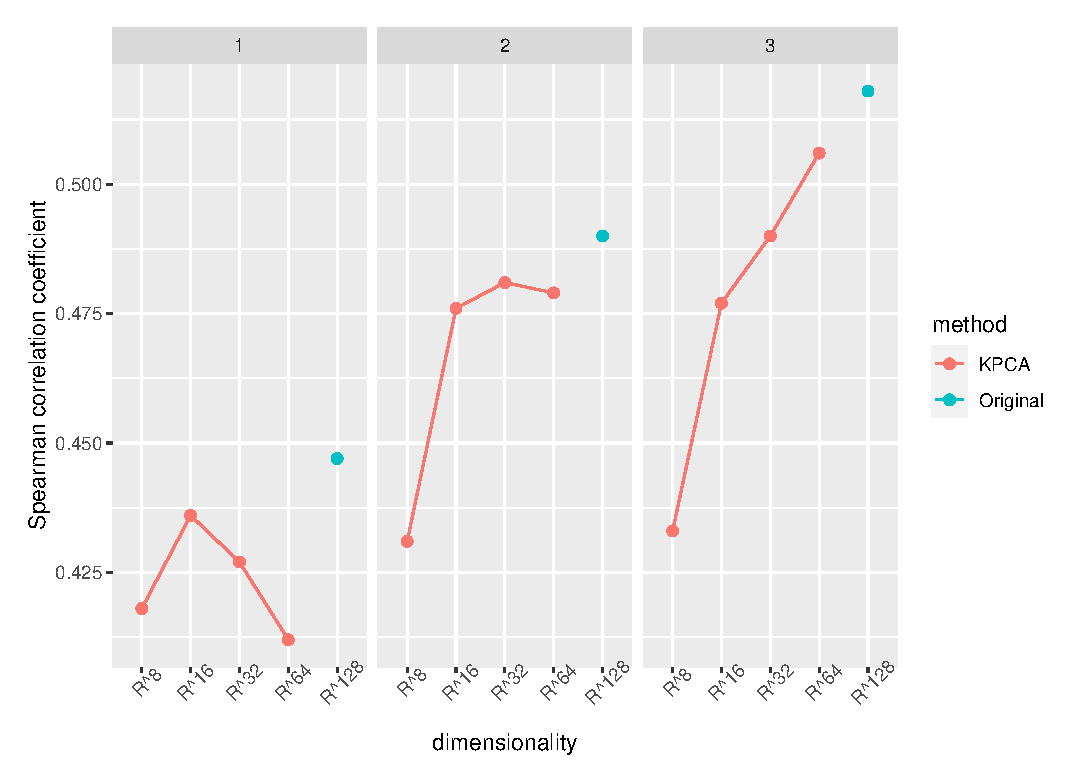
\includegraphics[width=12cm,height=7cm]{./Figures/spear_post.eps}
\caption{\textit{ex-post} KPCA: \textbf{Spearman correlation coefficient} of KPCA embeddings and original embeddings word2vec with state-of-the-art embeddings, for 1, 2, and 3 epochs. Higher is better.} 
\label{fig:spear_post}
\end{figure}






\pagebreak
\bibliographystyle{abbrv}
%\balance
\bibliography{ref}

\end{document}

% TODO
% - Previous work on kernels for NLP ◊
% - Use just KPCA as embeddings and see what happens ◊
% - Do a gridsearch on KPCA parameters ◊
% - Constrain word length ◊ --> future work
% - first most frequent then we removed less than 3 char ◊
% - 5 folds ◊
% - Write abstract  ◊
% - write future work  ◊
% - info on data (size?)  ◊
% - caption figures  ◊



% ---- BELANCHE'S SUGGESTIONS -----

%% TODO
% sqrt of distance (Tab 3) ◊
% captions! should describe clearly what tables/figures show ◊
% fix tables on sp correlation  ◊
% state questions clarly in intro (Hypothesis) ◊
% answer to research questions in conclusion 


%%% NOTES
% dot products are affected by dimensionality
% if you fit can you underfit or overfit?
% we care more about quick fit than accuracy
% careful not to generalize our results too much
% preprocess after data resampling
% if you formally define sth, then you should use it


%% FUTURE WORK
% dimens reduction on sentences
% what is the final application? --> best method depends on this
% different similarity measures
% different kernels?
% Constrain word length

%% WHAT TO EVALUATE
% number of hyperpars
% popssibility of doing feature selection
% computational cost of every run
% interpretability in addition to predictive performance
% --> understand rules


%-% Methodological Correctness
% global idea makes sense
% don't make any flaw